\documentclass[aspectratio=169,xcolor=dvipsnames]{beamer}
\makeatletter
\def\input@path{{theme/}}
\makeatother
\usetheme{CleanEasy}
\usepackage[utf8]{inputenc}
\usepackage{lmodern}
\usepackage[T1]{fontenc}
\usepackage{fix-cm}
\usepackage{amsmath}
\usepackage{mathtools}
\usepackage{listings}
\usepackage{xcolor}
\usepackage{hyperref}
\usepackage{graphicx}
\usepackage{booktabs}
\usepackage{tikz}
\usetikzlibrary{positioning, shapes, arrows, calc, decorations.pathreplacing, arrows.meta, backgrounds, patterns, overlay-beamer-styles, angles, quotes, intersections}
\usepackage{etoolbox}
\usepackage{animate}

\lstset{
  basicstyle=\ttfamily\small,
  keywordstyle=\color{blue},
  commentstyle=\color{green!60!black},
  stringstyle=\color{red},
  showstringspaces=false,
  breaklines=true,
  frame=single,
  rulecolor=\color{black!30},
  backgroundcolor=\color{black!5},
  numbers=left,
  numberstyle=\tiny\color{black!70},
  numbersep=5pt
}

%----------------------------------------------------------------------------------------
%    TITLE PAGE
%----------------------------------------------------------------------------------------

\title[Quadrilaterals]{Geometry: Circles}

\author[IA Math Team]{IA Math Team}

\vspace{-2cm}\date{Nov. 20, 2025}
%---------------------------------------------------------------------------------------

\begin{document}

\begin{frame}[t]
  \titlepage
\end{frame}

\begin{frame}[t]{Contents}
  \tableofcontents
\end{frame}

%----------------------------------------------------------------------------------------
\section{Warm-Up \& Recall}

\begin{frame}[t]{Circumference \& Area}
    \begin{definition}
    $\pi$ is defined as the ratio of the circumference of a circle to its diameter.
    \[
        \pi = \frac{\rm circumference}{\rm diameter}
    \]
    We also know that the area $=\pi r^2$ but why?
    \end{definition}
\end{frame}

\begin{frame}[t]{Fun Fact!}
    \vspace{2cm}
    \begin{center}
        \scalebox{3}{$\dfrac{d}{dr}(\pi r^2) = 2\pi r$}
    \end{center}
\end{frame}
\begin{frame}[t]{Lightning Quiz}
    If a circle has an area of $64\pi \;\text{cm}^2$, what would be the circumference of the circle?
    
    \vspace{2cm}
    
    If a circle has a circumference of $64\pi \;\text{cm}$, what would be the area?
\end{frame}

\section{Circles in Depth}

\begin{frame}[t]{Circle Anatomy}
  \begin{columns}[T,totalwidth=\textwidth]
    \begin{column}{0.45\textwidth}
      \begin{enumerate}
        \item Center
        \item Chord
        \item Diameter
        \item Sector
        \item Segment
        \item Arc
      \end{enumerate}
    \end{column}
    \begin{column}{0.55\textwidth}
      \begin{center}
        \begin{tikzpicture}[scale=1.1]
          \coordinate (O) at (0, 0);
          \draw (O) circle (2);
        \end{tikzpicture}
      \end{center}
    \end{column}
  \end{columns}
\end{frame}



\begin{frame}[t]{More Angles}

\begin{center}
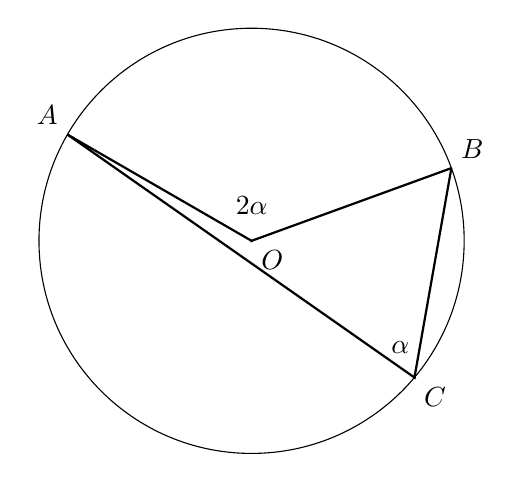
\begin{tikzpicture}[scale=1.8]
  % Circle and center
  \coordinate (O) at (0,0);
  \draw (O) circle (1.5);

  % Points on the circle
  \coordinate (A) at (150:1.5);
  \coordinate (B) at (20:1.5);
  \coordinate (C) at (-40:1.5);

  % Radii for central angle
  \draw[thick] (O) -- (A);
  \draw[thick] (O) -- (B);

  % Inscribed angle at C
  \draw[thick] (A) -- (C) -- (B);

  % Angle arcs only (no text attached)
  \pic [draw, angle radius=0.35] {angle = A--O--B};
  \pic [draw, angle radius=0.35] {angle = A--C--B};

  % Labels placed manually, outside the "triangle" regions
  \node at (0,0.25) {$2\alpha$};   % near central angle arc
  \node at (1.05,-0.75) {$\alpha$};  % near inscribed angle arc

  % Point labels
  \node[above left]  at (A) {$A$};
  \node[above right] at (B) {$B$};
  \node[below right] at (C) {$C$};
  \node[below right] at (O) {$O$};
\end{tikzpicture}
\end{center}

Here, we have that $\angle AOB=2\angle ACB$. How do we get this?
\end{frame}

\begin{frame}[t]{Usain Bolt Quiz}
On Circle U, we have points S and I which form a diameter. We also have a point A somewhere random on the circumference of the circle other than S or I. If points S, A, I form angle N, what is the degree measure of N?
\end{frame}

\begin{frame}[t]{Tangents}
    \begin{definition}
        A tangent line to a circle is one that intersects it at exactly one point.
    \end{definition}

    \vspace{0.67cm}
    \begin{center}
    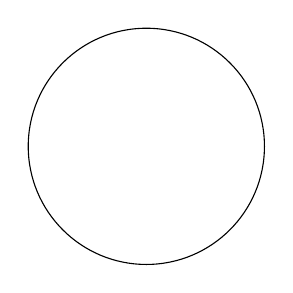
\begin{tikzpicture}[scale=1]
        \coordinate (O) at (0,-2);
        \draw (O) circle (1.5);
    \end{tikzpicture}
    \end{center}
\end{frame}


\begin{frame}{Power of a Point}

\begin{center}
\begin{tikzpicture}[scale=1.67]
  % Circle and center
  \coordinate (O) at (0,0);
  \draw (O) circle (1.5);
\end{tikzpicture}
\end{center}

\end{frame}

\section{Worksheet}



\end{document}
